\chapter{Contexte d'étude et revue de littérature}

\section{Problématique}
La république du Bénin est située en Afrique occidentale et fait partie des Etats côtier du Golfe du Guinée. Malgré ses dimensions réduites elle recèle d’importants attraits touristiques qui varient du sud au nord. De ce fait les flux touristiques vers le Bénin augmentent chaque année. En effet, la croissance est soutenue et est de l'ordre de 4\% depuis 1992\footnote{Jean-Philippe Principaud, « Le tourisme international au Bénin : une activité en pleine expansion », Les Cahiers d’Outre-Mer, 226-227 | 2004, 191-216.}. Les derniers chiffres officiels, pour la saison 2014-2015 tablent sur une affluence de 200 000 touristes. La construction de plus en plus d’établissements d’hébergement et les arrivés fréquentes de voyageurs dans ces établissement confirment cette affluence. De plus, d'après l’Agence Nationale de Promotion des patrimoines et du développement du Tourisme (ANPT), entre 2017-2021 un investissement de 600 milliards de francs Cfa est prévu pour le tourisme avec pour objectif d'attirer au moins 700 000 touristes d’ici 2021\footnote{Présidence-Bénin. « Programme d'actions du gouvernement 2016-2021 Synthèse ». Bénin Révélé, 28 | 2017.}. Pourtant le logement au Bénin reste une difficulté, même pour les nationaux.

En effet, peu d’agences de voyage sont informatisées. La plupart des touristes à leur arrivée sont confrontés au manque de logement de qualite libres. Aussi, devant visiter plusieurs villes durant leur séjour, il leur faut un accueil chaleureux et une expérience remarquable à chaque escale, ce qui est rarement le cas.

D'autre part, on observe les difficultés auxquelles sont confrontées les populations béninoises pour trouver un logement quand ils sont en déplacement d’une ville à une autre.

Ces problèmes recensés reflètent d’une manière générale, un problème de manque d’informations accessibles rapidement et gratuitement à tous en ce qui concerne les secteurs de l’habitat du tourisme et de la culture.

De tout ce qui précède, il se pose la question de trouver un moyen de communication moderne et efficace pour mettre en contact un hôte local et un voyageur à la quête d'un logement convivial à prix raisonnable ou d'une expérience unique. Il s’agit non seulement  d'aider les voyageurs à trouver le logement qui leur convient mais aussi de leur faire découvrir des lieux et participer à des expériences inoubliables. Ceci permettra de garantir une expérience de voyage de qualité. D’où l’intérêt de recourir aux Technologies de l’Information et de la Communication (TIC) afin de proposer des logements uniques à travers le Bénin, de les découvrir et de les réserver à l’avance.




\section{Objectifs}
La plateforme à réaliser sera un véritable outil qui permettra de proposer des logements uniques à travers le Bénin, de les découvrir et de les réserver ; en ligne, sur un téléphone mobile ou une tablette.
\\Qu'il s'agisse d'un appartement pour une nuit ou d'une villa pour un mois, l’application offrira des expériences de voyage exceptionnelles, à tous les prix, dans toutes les villes du pays.

\section{État de l’art} 

\subsection{Présentation des solutions existantes} 
Il existe plusieurs solutions pour la location de courte durée d’appartement ou de parties d’appartement en ligne. Il s’agit notamment de:

\paragraph{Airbnb : Le leader}
$ $
\begin{figure}[H]
\begin{center}

\includegraphics[width=6.5cm]{images/concurrent/airbnb3.png}
\end{center}
\caption{Logo Airbnb}
\end{figure}
$ $
Airbnb  \footnote{https://airbnb.com/} permet à des particuliers de louer tout ou une partie de leur propre habitation comme logement d'appoint. Le site offre une plateforme de recherche et de réservations entre la personne qui offre son logement et le vacancier qui souhaite le louer. Il couvre plus de 1,5 million d'annonces dans plus de 34 000 villes et 191 pays.
\\Il est le leader du marché. En effet, de sa création, en août 2008, jusqu'en juin 2012, plus de 10 millions de nuits ont été réservées sur Airbnb.
\newpage
\begin{figure}[H]
\begin{center}
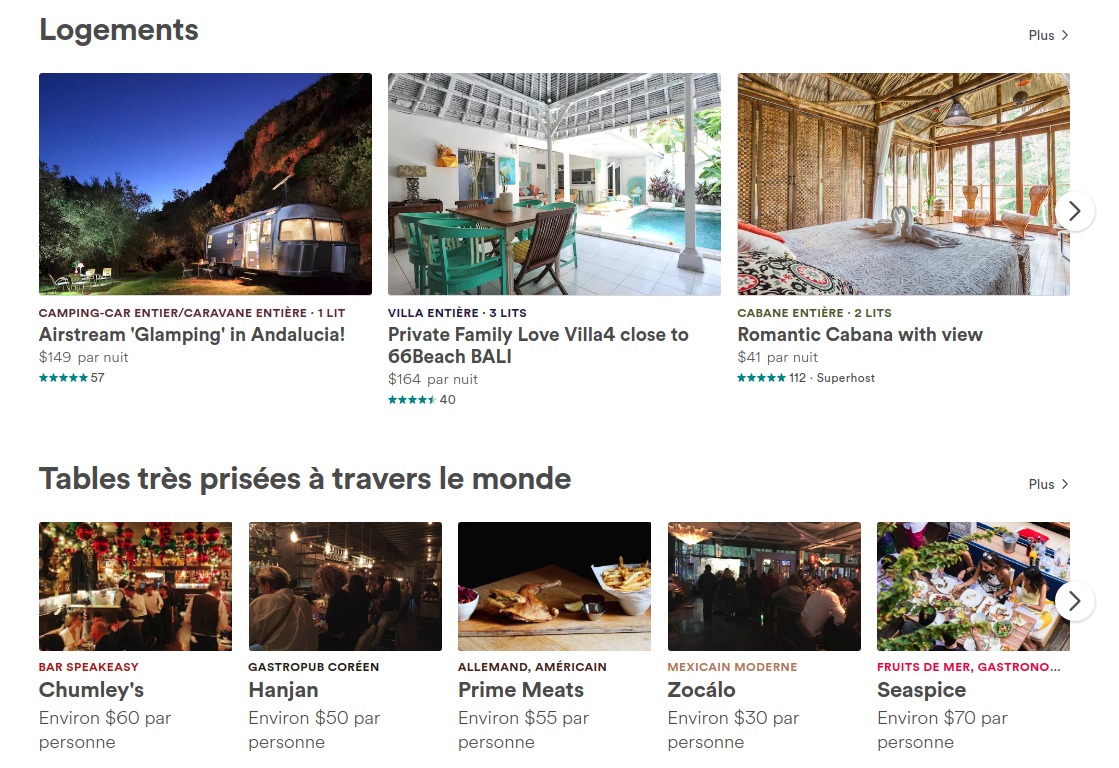
\includegraphics[width=17.5cm]{images/concurrent/airbnb1.png}
\end{center}
\caption{Accueil Airbnb}
\end{figure}

\paragraph{Les alternatives }
$ $\\Il s’agit de :
\begin{itemize}
\item[\textbullet] Tripping.com
\item[\textbullet] Booking.com
\item[\textbullet] Homeaway
\item[\textbullet] VRBO
\item[\textbullet] Trivago
\item[\textbullet] Outdoorsy
\item[\textbullet] Homestay
\item[\textbullet] Hotels.com
\item[\textbullet] Expedia
\item[\textbullet] Roomorama (ferme)
\item[\textbullet] Flipkey
\end{itemize}

\newpage
\begin{figure}[H]
\begin{center}

\includegraphics[width=17cm]{images/concurrent/airalt1.png}
\end{center}
\caption{Logos concurrents}
\end{figure}

Elles sont, pour la plupart nées suite à l’engouement autour de Airbnb. Ces plateformes proposent pêle-mêle : la location sur courte ou longue durée, la comparaison d’offres entre différentes plateformes, ...
\\Elles sont orientés exclusivement vers les marchés européen et américain.

\paragraph{Au Bénin : BeninMaison et BeninImmo}
$ $
\begin{figure}[H]
    \begin{minipage}[c]{.46\linewidth}
        \centering
        
\includegraphics[width=6.3cm]{images/concurrent/beninimmo2.png}
        \caption{Logo BeninImmo}
    \end{minipage}
    \hfill%
    \begin{minipage}[c]{.46\linewidth}
        \centering
        
\includegraphics[width=6.5cm]{images/concurrent/beninmaison2.png}
        \caption{Logo BeninMaison}
    \end{minipage}
\end{figure}

$ $
Ces plateformes  \footnote{https://beninmaison.com/, http://www.benin-immo.com/} proposent des services tel que:
\begin{itemize}
\item[\textbullet] Faire estimer un bien
\item[\textbullet] Mettre un bien en vente
\item[\textbullet] Mettre en location
\item[\textbullet] Acheter un bien immobilier
\item[\textbullet] Louer un logement
\item[\textbullet] Faire gérer son bien
\end{itemize}

\newpage
\begin{figure}[h]
\begin{center}
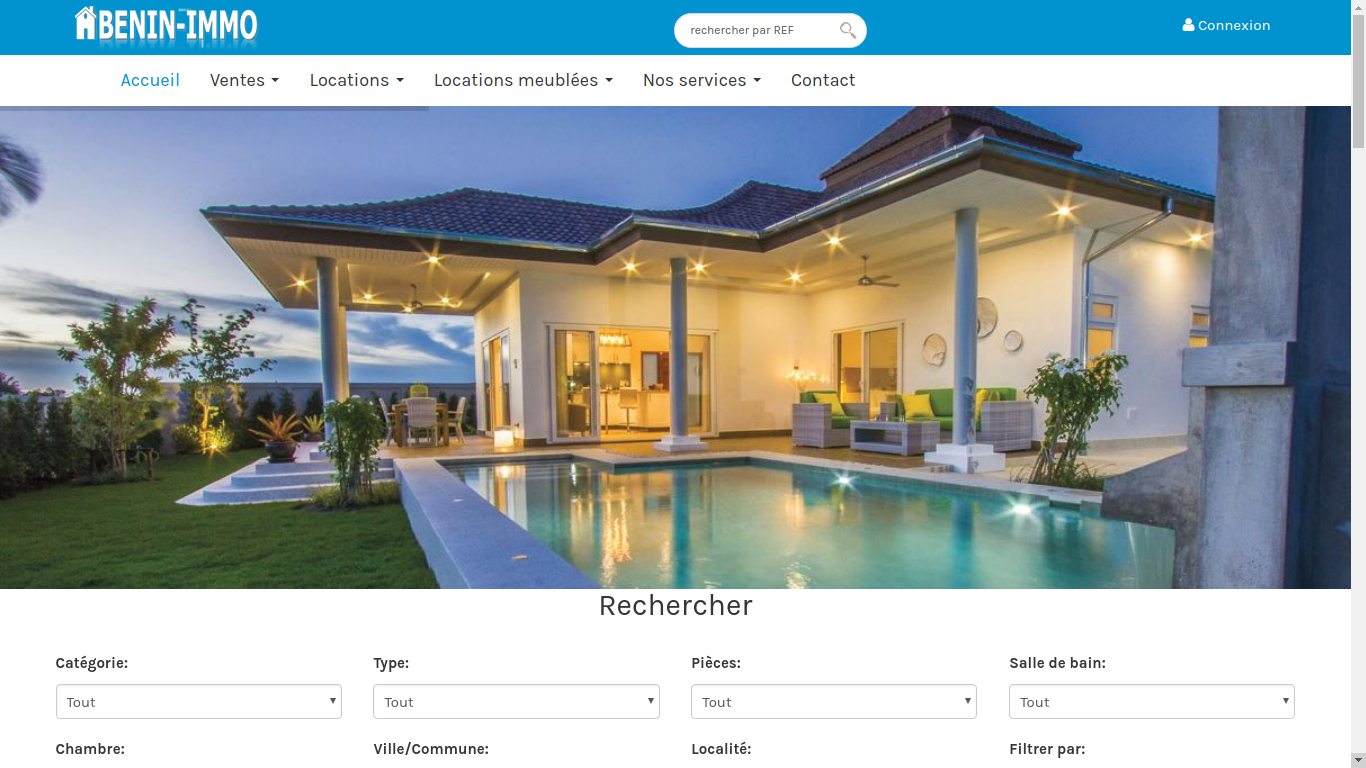
\includegraphics[width=17cm]{images/concurrent/beninimmo1.png}
\end{center}
\caption{Accueil BeninImmo}
\end{figure}

$\phantom{11111111111111111} $ $\phantom{11111111111111111}$
\begin{figure}[H]
\begin{center}

\includegraphics[width=17cm]{images/concurrent/beninmaison1.png}
\end{center}
\caption{Accueil BeninMaison}
\end{figure}

\newpage
\subsection{Intérêt de la solution par rapport aux existantes} 
Le leader du marché ainsi que ses concurrents occidentaux, orientent principalement leurs services vers les villes européennes et américaines. On note ainsi une très faible quantité d’offres provenant du Bénin.
\\Les plateformes béninoises quant à elles ont du mal à émerger. On citera entre autres comme problèmes observés :
\begin{itemize}
\item[\textbullet] la pauvreté de l’offre ;
\item[\textbullet] une UI\footnote{User Interface} très peu attrayante ;
\item[\textbullet] le manque ou l’absence de communication ;
\item[\textbullet] l’absence de moyen de paiement en ligne adapté ;
\subitem[\textbullet] Transactions internationales: Impossibilité de recevoir de l’argent sur un compte béninois via Paypal;
\subitem[\textbullet] Transactions locales : Faible bancarisation de la population locale, difficultés d’accès aux api MTN et MOOV mobile money;
\item[\textbullet] l’absence de location courte durée, et de la possibilité de louer une partie de son bien immobilier.
\end{itemize}

Avec notre application, les utilisateurs pourront réserver très rapidement un grand nombre de logements dans toutes les villes du Bénin. Ils pourront également vivre des expériences particulières avec un hôte de leur ville d'accueil. Une attention particulière sera accordée à l’interface d’utilisateur ainsi qu'à l'expérience d’utilisateur aussi bien sur la plateforme que sur le terrain par les commentaires et les notes.